\documentclass[journal,12pt,twocolumn]{IEEEtran}

\usepackage{setspace}
\usepackage{gensymb}
\singlespacing
\usepackage[cmex10]{amsmath}

\usepackage{amsthm}

\usepackage{mathrsfs}
\usepackage{txfonts}
\usepackage{stfloats}
\usepackage{bm}
\usepackage{cite}
\usepackage{cases}
\usepackage{subfig}

\usepackage{longtable}
\usepackage{multirow}

\usepackage{enumitem}
\usepackage{mathtools}
\usepackage{steinmetz}
\usepackage{tikz}
\usepackage{circuitikz}
\usepackage{verbatim}
\usepackage{tfrupee}
\usepackage[breaklinks=true]{hyperref}
\usepackage{graphicx}
\usepackage{tkz-euclide}

\usetikzlibrary{calc,math}
\usepackage{listings}
    \usepackage{color}                                            %%
    \usepackage{array}                                            %%
    \usepackage{longtable}                                        %%
    \usepackage{calc}                                             %%
    \usepackage{multirow}                                         %%
    \usepackage{hhline}                                           %%
    \usepackage{ifthen}                                           %%
    \usepackage{lscape}     
\usepackage{multicol}
\usepackage{chngcntr}

\DeclareMathOperator*{\Res}{Res}

\renewcommand\thesection{\arabic{section}}
\renewcommand\thesubsection{\thesection.\arabic{subsection}}
\renewcommand\thesubsubsection{\thesubsection.\arabic{subsubsection}}

\renewcommand\thesectiondis{\arabic{section}}
\renewcommand\thesubsectiondis{\thesectiondis.\arabic{subsection}}
\renewcommand\thesubsubsectiondis{\thesubsectiondis.\arabic{subsubsection}}


\hyphenation{op-tical net-works semi-conduc-tor}
\def\inputGnumericTable{}                                 %%

\lstset{
%language=C,
frame=single, 
breaklines=true,
columns=fullflexible
}
\begin{document}

\newcommand{\BEQA}{\begin{eqnarray}}
\newcommand{\EEQA}{\end{eqnarray}}
\newcommand{\define}{\stackrel{\triangle}{=}}
\bibliographystyle{IEEEtran}
\raggedbottom
\setlength{\parindent}{0pt}
\providecommand{\mbf}{\mathbf}
\providecommand{\pr}[1]{\ensuremath{\Pr\left(#1\right)}}
\providecommand{\qfunc}[1]{\ensuremath{Q\left(#1\right)}}
\providecommand{\sbrak}[1]{\ensuremath{{}\left[#1\right]}}
\providecommand{\lsbrak}[1]{\ensuremath{{}\left[#1\right.}}
\providecommand{\rsbrak}[1]{\ensuremath{{}\left.#1\right]}}
\providecommand{\brak}[1]{\ensuremath{\left(#1\right)}}
\providecommand{\lbrak}[1]{\ensuremath{\left(#1\right.}}
\providecommand{\rbrak}[1]{\ensuremath{\left.#1\right)}}
\providecommand{\cbrak}[1]{\ensuremath{\left\{#1\right\}}}
\providecommand{\lcbrak}[1]{\ensuremath{\left\{#1\right.}}
\providecommand{\rcbrak}[1]{\ensuremath{\left.#1\right\}}}
\theoremstyle{remark}
\newtheorem{rem}{Remark}
\newcommand{\sgn}{\mathop{\mathrm{sgn}}}
\newcommand{\comb}[2]{{}^{#1}\mathrm{C}_{#2}}
\providecommand{\abs}[1]{\vert#1\vert}
\providecommand{\res}[1]{\Res\displaylimits_{#1}} 
\providecommand{\norm}[1]{\lVert#1\rVert}
%\providecommand{\norm}[1]{\lVert#1\rVert}
\providecommand{\mtx}[1]{\mathbf{#1}}
\providecommand{\mean}[1]{E[ #1 ]}
\providecommand{\fourier}{\overset{\mathcal{F}}{ \rightleftharpoons}}
%\providecommand{\hilbert}{\overset{\mathcal{H}}{ \rightleftharpoons}}
\providecommand{\system}{\overset{\mathcal{H}}{ \longleftrightarrow}}
	%\newcommand{\solution}[2]{\textbf{Solution:}{#1}}
\newcommand{\solution}{\noindent \textbf{Solution: }}
\newcommand{\cosec}{\,\text{cosec}\,}
\providecommand{\dec}[2]{\ensuremath{\overset{#1}{\underset{#2}{\gtrless}}}}

\newcommand{\myvec}[1]{\ensuremath{\begin{pmatrix}#1\end{pmatrix}}}
\newcommand{\mydet}[1]{\ensuremath{\begin{vmatrix}#1\end{vmatrix}}}
\numberwithin{equation}{subsection}
\makeatletter
\@addtoreset{figure}{problem}
\makeatother
\let\StandardTheFigure\thefigure
\let\vec\mathbf
\renewcommand{\thefigure}{\theproblem}
\def\putbox#1#2#3{\makebox[0in][l]{\makebox[#1][l]{}\raisebox{\baselineskip}[0in][0in]{\raisebox{#2}[0in][0in]{#3}}}}
     \def\rightbox#1{\makebox[0in][r]{#1}}
     \def\centbox#1{\makebox[0in]{#1}}
     \def\topbox#1{\raisebox{-\baselineskip}[0in][0in]{#1}}
     \def\midbox#1{\raisebox{-0.5\baselineskip}[0in][0in]{#1}}
\vspace{3cm}
\title{Assignment 2}
\author{Challa Akshay Santoshi-CS21BTECH11012}
\maketitle
\newpage
\bigskip
\renewcommand{\thefigure}{\theenumi}
\renewcommand{\thetable}{\theenumi}
\begin{center}
  \textbf{\underline{ICSE 12 2019}}\\
\end{center}
\begin{center}
  \textbf{Question: 20 (b)}  
\end{center}
Find the equation of the regression line of y on x, if the observations (x, y) are as follows:\\
(1, 4), (2, 8), (3, 2), (4, 12), (5, 10), (6, 14), (7, 16), (8, 6), (9, 18)\\
Also find the estimated value of y when x = 14.\\
\begin{center}
  \textbf{Solution:}  
\end{center}
Let the regression line of y on x be given as\\
\begin{align}
    \myvec{a_1 & -1}\vec{Z} = a_0
\end{align}
Here, $\vec{Z} = \myvec{x\\y}$.
The observations given can be written as follows\\
\begin{align}
		 \myvec{x_1\\y_1},\myvec{x_2\\y_2}.....,\myvec{x_n\\y_n}
\end{align}
Let us define few matrices as follows\\
\begin{align}   
	      	\vec{Y}&=\myvec{y_1\\y_2\\.\\.\\y_{n-1}\\y_n},
	      	\vec{X}=\myvec{1&x_1\\1&x_2\\.&\\.&\\1&x_{n-1}\\1&x_n}
	      	\\
	      	\vec{A}&=\myvec{a_1\\a_0},
	      	\vec{E}=\myvec{e_1\\e_2\\.\\.\\e_{n-1}\\e_n}\\
      		\vec{E}=&\vec{Y}-\vec{X}\vec{A}
\end{align}
$ \vec{E}$ is the matrix of residual errors.\\
To get the regression line which is the best fit line equation for a given data, the sum of squares of residual errors has to be minimum.\\
Let SSE be the sum of square of errors.\\
\begin{align}
      	SSE&=\norm{\vec{E}^{\top}\vec{E}}\\ &=\brak{\vec{Y}-\vec{X}\vec{A}}^{\top}\brak{\vec{Y}-\vec{X}\vec{A}}\\
      	&=\brak{\vec{Y}^{\top}-\vec{A}^{\top}\vec{X}^{\top}}\brak{\vec{Y}-\vec{X}\vec{A}}
      	\\
      	&=\brak{\vec{Y}^{\top}\vec{Y}-\vec{Y}^{\top}\vec{X}\vec{A}-\vec{A}^{\top}\vec{X}^{\top}\vec{Y}+\vec{A}^{\top}\vec{X}^{\top}\vec{X}\vec{A}}
\end{align}
$ \vec{Y}^{\top}\vec{X}\vec{A} $ is of order $ \brak{1 \times 1} $. Therefore it is equal to its transpose.
\begin{align}
    \vec{Y}^{\top}\vec{X}\vec{A} &= \brak{\vec{Y}^{\top}\vec{X}\vec{A}}^{\top}\\
    &= \vec{A}^{\top}\vec{X}^{\top}\vec{Y}
\end{align}
This will give,
\begin{align}
    SSE = \brak{\vec{Y}^{\top}\vec{Y}-2\vec{A}^{\top}\vec{X}^{\top}\vec{Y}+\vec{A}^{\top}\vec{X}^{\top}\vec{X}\vec{A}}
\end{align}\\
For SSE to be minimum, take the gradient with respect to A.
\begin{align}
      	 \nabla
      		SSE
      		&=\brak{\nabla\vec{Y}^{\top}\vec{Y}-2\nabla\vec{A}^{\top}\vec{X}^{\top}\vec{Y}+\nabla\vec{A}^{\top}\vec{X}^{\top}\vec{X}\vec{A}}\\
      		&=2\brak{\vec{X}^{\top}\vec{X}\vec{A}-\vec{X}^{\top}\vec{Y}}
\end{align}
Equate it to zero to get the minimum condition.
\begin{align}
       \brak{\vec{X}^{\top}\vec{X}\vec{A}-\vec{X}^{\top}\vec{Y}}=0\\
       \vec{A}=\brak{\vec{X}^{\top}\vec{X}}^{-1}\vec{X}^{\top}\vec{Y}
\end{align}\\
Using data given in question\\
\begin{align}
	\myvec{x \\y }:
	\myvec{1 \\4 },
	\myvec{2 \\8 },
	\myvec{3 \\2 },
    \myvec{4 \\12 },
    \myvec{5 \\10 },
    \myvec{6 \\14 },
    \myvec{7 \\16 },
    \myvec{8 \\6 },
    \myvec{9 \\18 }
\end{align}
\begin{align}
	\vec{Y}=\myvec{4\\8\\2\\12\\10\\14\\16\\6\\18},
	\vec{X}=\myvec{1&1\\1&2\\1&3\\1&4\\1&5\\1&6\\1&7\\1&8\\1&9}
\end{align}
Using equations (0.0.16) and (0.018), solving will give
\begin{align}
	A=\myvec{\frac{10}{3}\\\frac{4}{3}}
\end{align}
Using equation (0.0.1), regression line equation can be obtained.
\begin{align}
    \myvec{\frac{4}{3} & -1}\myvec{x\\y}= \frac{10}{3}
\end{align}
From this equation we get the value of y as 22 when x is 14.\\
\begin{figure}[ht]
    \centering
    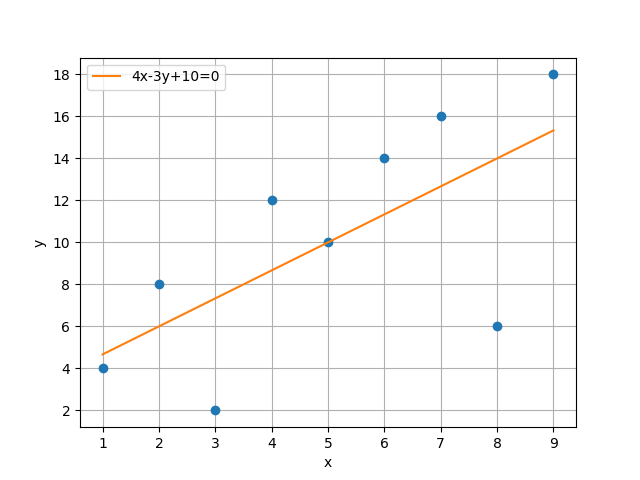
\includegraphics[width=\columnwidth]{Figure_1.png}
    \caption{Graph showing the Regression Line}
    \label{Figure_1}
\end{figure}\\
\end{document}